The first subsection will explain the system's architecture in detail based on a \ac{UML} diagram. With this diagram, it is possible to show the component-based architecture and how the mentioned tools are combined for the different visualisations and concepts. The second subsection will show the transition manager in detail, which features the transition table mentioned in chapter \ref{s:theoretical-contrib} on page \pageref{s:theoretical-contrib}.
As already mentioned in chapter \ref{s:collaboration-statement} on page \pageref{s:collaboration-statement}, \citeauthor{Wanko2016} is researching on a related topic of this thesis. The practical part of his his thesis and the one of this thesis are implemented in the same system. Therefore, the actual application has a lot more features and options than described in this section.

\subsubsection{Application Architecture}
Figure \ref{fig:uml-practical-approach} on page \pageref{fig:uml-practical-approach} gives an overview of the architecture in the form of a class diagram. However, the diagram shown and discussed in the master-thesis of \citeauthor{Wanko2016} looks quite different, although it is based on the same system. This is due to the relatively big system architecture and the different scopes of both theses \iacite{Wanko2016}. Showing and discussing all available classes, features and options for the application would go beyong the scope. The following list will briefly discuss the most important classes and their purposes:

%TC:ignore
\begin{figure}[!htb]
\centering
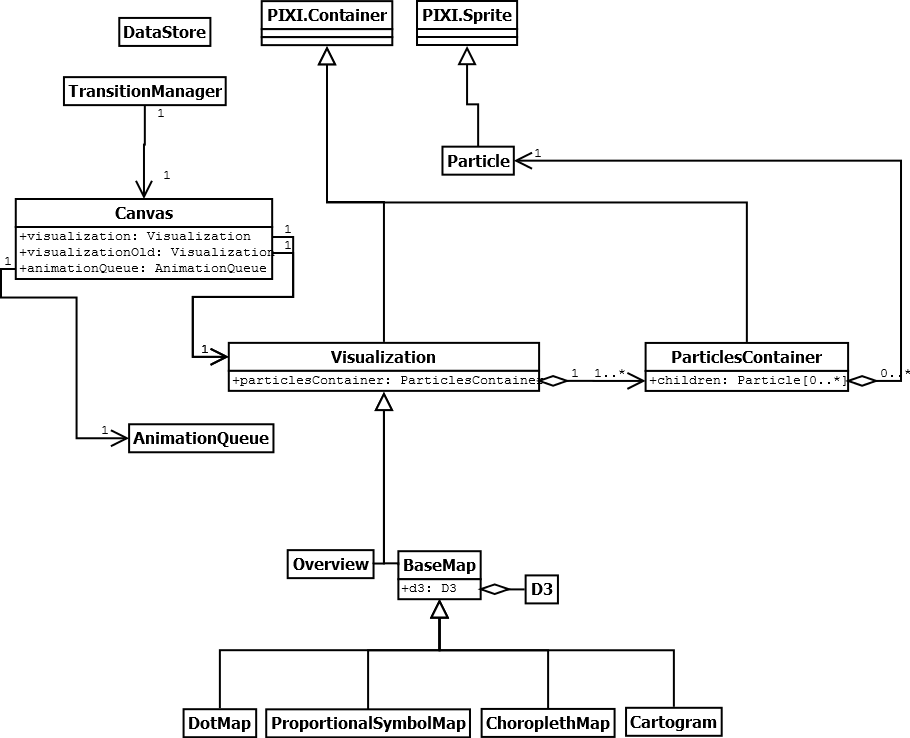
\includegraphics[width=0.8\textwidth,keepaspectratio]{images/results/dia.png}
\caption[
    Overview of the application architecture in the form of a class diagram.
]{Overview of the application architecture in the form of a class diagram.}
\label{fig:uml-practical-approach}
\end{figure}
%TC:endignore

\begin{description}
\item[DataStore] \hfill \\
An object of the DataStore-class is used to load the SuperStore-Sale dataset. In addition to initally loading it, it also parses and analyses the dataset. Each attribute of the dataset got classified to handle the attributes correctly later on. For the sake of convenience, three different classification types were used: numeric, date, nominal and unknown.

\item[PIXI.Container] \hfill \\
\ac{Pixi} features functionalities like container classes. \textit{PIXI.Container} is such a class and can be used to put objects in it, and scale or move those objects according to the base-canvas.

\item[AnimationQueue] \hfill \\
If an animation is assigned to particles, it is stored in the \textit{AnimationQueue}. This allows to create multiple canvas-based animations and process them sequential.

\item[Canvas] \hfill \\
This class is one of the main classes inside the application. It is needed to not compare it with an HTML-Canvas object. However, this class is responsible for creating the base-canvas of the web-application. Furthermore, it is used to change and update the visual appearance if any interaction happens. A key part of the canvas class is the render function shown in listing \ref{lst:canvas-render} on page \pageref{lst:canvas-render}. It starts off with calling the same function again as soon as possible. The caller-function \textit{requestAnimationFrame} ensures, that the next frame will only be shown if enough resources of the browser are available. Afterwards, all particles and visualisations are animated if something changed. The last line of the listing shows the \ac{Pixi}-renderer. Listing \ref{lst:canvas-autodecet-renderer} on page \pageref{lst:canvas-autodecet-renderer} shows its creation. It features the main canvas-size, background transparency, antialiasing and a lot of other options.

%TC:ignore
\begin{lstlisting}[language=JavaScript, caption={Render function of the canvas class.}, label={lst:canvas-render}]
    render() {
      this.requestFrameID = requestAnimationFrame(this.render.bind(this));

      let areParticlesAnimating = this.particlesContainer.nextStep();
      let isNewVisualizationAnimating = this.visualization.nextStep();
      let isOldVisualizationAnimating =  ? this.visualizationOld.nextStep() : false;

      if (!areParticlesAnimating && !isOldVisualizationAnimating &&
        !isNewVisualizationAnimating && this.animationQueue.length > 0) {

        this.animationQueue.pop()();
        this.particlesContainer.startAnimation();
        this.visualization.startAnimation();
        if (this.visualizationOld){
            this.visualizationOld.startAnimation();
        }
      }
      this.renderer.render(this.stage);
    }
\end{lstlisting}

\begin{lstlisting}[language=JavaScript, caption={Pixi's autodetect-renderer.}, label={lst:canvas-autodecet-renderer}]
    this.renderer = PIXI.autoDetectRenderer(this.width, this.height, {
        transparent: true,
        clearBeforeRender: true,
        antialias: true
    });
    document.body.appendChild(this.renderer.view);
\end{lstlisting}
%TC:endignore

\item[Visualization] \hfill \\
This class is the starting point and the parent class for all other types of visualisations. It stores a reference to the \textit{ParticleContainer} and provides functionality to move, scale or change visualisations.

\item[Overview] \hfill \\
Creating an instance of \textit{Overview} will show all data items as unit-based grid.

\item[D3] \hfill \\
This class is mainly used to wrap all functionality of the \ac{D3} library. It features functions like initialising the base-map as a \ac{SVG} and loading the needed TopoJSON data accordingly. \ac{D3} offers multiple projections for GeoJSON data. Listing \ref{lst:d3-map-init} on page \pageref{lst:d3-map-init} shows a part of the map initialisation with the projection used. The projection is an extension of an Albers equal-area projection discussed in chapter \ref{s:map-projections} on page \pageref{s:albers-equal-area-projection}. It is a United-States-centric composite projection. The lower forty-eight states of america are projected using the default Albers-equal-area projection. However, Alaska and Hawaii use a separate conic equal-area projection. The scale of Alaska is furthermore diminished. It is projected at $0.35\times$ its true relative area. The scale and translation of the map are set to use the available window space and center the map on the screen.

%TC:ignore
\begin{lstlisting}[language=JavaScript, caption={Map initialisation with a map projection, scale, and translation.}, label={lst:d3-map-init}]
    this.projection = this._d3.geo.albersUsa()
        .scale(width)
        .translate([this.width / 2, this.height / 2]);
\end{lstlisting}
%TC:endignore

Another key part of this class is featured in listing \ref{lst:d3-topojson} on page \pageref{lst:d3-topojson}. It shows how TopoJSON is used on the client. The filter function passed to the first \textit{TopoJSON.mesh}-function specifies that only internal state borders should be drawn. Thus, coastlines will not be drawn to retain detail around small islands and inlets. The filter function passed to the second \textit{TopoJSON.mesh}-function extends the first one by only drawing each county boundary once. Thus, if two counties share the same border, it is only drawn once.

%TC:ignore
\begin{lstlisting}[language=JavaScript, caption={TopoJSON usage on the client with the adaption of merging all geographic information.}, label={lst:d3-topojson}]
    this.data.topojson.states = topojson.mesh(
        this.data.us,
        this.data.us.objects.states,
        (a, b) => {
            return a !== b;
        }
    );

    this.data.topojson.counties = topojson.mesh(
        this.data.us,
        this.data.us.objects.counties,
        (a, b) => {
            return (
                a !== b &&
                !(this.getCountyIdentifier(a) / 1000 ^ this.getCountyIdentifier(b) / 1000)
            );
        }
    );
\end{lstlisting}
%TC:endignore

Another important aspect of the \ac{D3} class is the \textit{calculateCentroids}-function shown in listing \ref{lst:d3-calculate-centroids} on page \pageref{lst:d3-calculate-centroids}. It calculates a look-up dictionary for the given level of detail for each data item. Thus, providing a huge performance boost when finding out the centroid of a unit later on.

%TC:ignore
\begin{lstlisting}[language=JavaScript, caption={Calculate a look-up dictionary for all data items depending on the level of detail.}, label={lst:d3-calculate-centroids}]
    calculateCentroids(levelOfDetail){
        const boundaries = this._topojson.feature(
            this.data.us,
            this.data.us.objects[levelOfDetail]
        ).features;

        this.centroids[levelOfDetail] = {};
        for(let boundary of boundaries){
            this.centroids[levelOfDetail][boundary.id] = this.path.centroid(boundary);
        }
    }
\end{lstlisting}
%TC:endignore

% SYMBOL SCALE AND COLOR SCALE TO SHOW

\item[BaseMap] \hfill \\
This is the second class inheriting from the \textit{Visualization} class. It features a single object of the \ac{D3} class. Therefore, it is possible that all deriving classes share the same object of \ac{D3} and thus, all its features and settings. Changing the level of detail of the \textit{BaseMap} will affect the map initialised in \textit{\ac{D3}} and hence, all deriving classes are using the same base-map again. This class is mainly used to share the same object of \ac{D3} for all children.
The decision if the upcoming map should be animated or not handles each subclass on its own. All of them use the same concept of determining the type of transition: each implemented subclass has some kind of \textit{draw}-function which accepts an optional parameter called \textit{animationCb}. If this parameter exists and is not \textit{undefined}, the transition to the upcoming visualisation is animated.
All subclasses based on aggregation are implemented and animated with \ac{D3}. Therefore, dot map is slightly different than these in the terms of structure and usage. Furthermore, all thematic maps based on aggregation are implemented with the method of using a static file consisting of all information. However, the aggregated values could also be calculated every time.

\item[DotMap] \hfill \\
The \textit{DotMap} class is the first one to show data on the base-map. It does not use the \ac{DOM} to create the units on the map. It uses the already existing particles from the particle container inherited from the \textit{Visualization} class. Key part of this class is the determination of animating particles or not.
The herein before mentioned decision if particle should be animated or not is shown in listing \ref{lst:dot-draw-animated} on page \pageref{lst:dot-draw-animated}. It also shows the further executed actions if they should be animated, like projecting the longitude and latitude of the point onto the map and calling the main \textit{draw}-function for each particle.

%TC:ignore
\begin{lstlisting}[language=JavaScript, caption={Particles on a dot map getting animated.}, label={lst:dot-draw-animated}]
    if(this.isFunction(animationCb)){
        for(let particle of this.particles){
            point = [particle.data.Longitude, particle.data.Latitude];
            point = this.baseMap.projection(point);
            particle.coords = point;

            setTimeout(drawFunc.bind(this), 250, particle, this.size);
        }
    }
\end{lstlisting}
%TC:endignore

\item[ProportionalSymbolMap] \hfill \\
Drawing proportional symbols is done by using \ac{D3}. First of all, it does not use the SuperStore-Sale file as a basis, and instead uses the preprocessed TopoJSON file. The \textit{draw}-function of this class gets two parameters: the level of detail which should be drawn and the decision if the symbols should be animated. Listing \ref{lst:psm-draw} on page \pageref{lst:psm-draw} shows how each circle for the proportional symbol map is drawn and eventually animated. Line 8-13 loads the already existing data into the created \ac{SVG}-element. It is important to sort the data first because if this would not happen, bigger circles would cover smaller ones. Drawing the bigger ones first results in zero overpainting. The \textit{.data()}-function returns an array. Iterating through every item in the array is done with the \textit{.enter()}-method. Line 15 and onwards create a proportional symbol called \textit{circle} for each data item in the array. They set its position with \textit{transform} and decide, if its radius should be animated or not.

%TC:ignore
\begin{lstlisting}[language=JavaScript, caption={The draw-function of the ProportionalSymbolMap-class}, label={lst:psm-draw}]
    draw(id, animationCb){
        let map = this.baseMap;

        this[id] = map.svg.append("g")
        .attr("id", `psm-${id}`)
        .attr("class", "bubble")
        .selectAll("circle")
        .data(
            map._topojson.feature(map.data.us, map.data.us.objects[id]).features
            .sort(function(a, b) {
                return (b.properties.orders || 0) - (a.properties.orders || 0);
            })
        )
        .enter()
        .append("circle")
        .attr("transform", function(d) {
            let coords = map.path.centroid(d);
            if(isNaN(coords[0]) || isNaN(coords[1])) return;
            return "translate(" + coords + ")";
        });

        if(this.isFunction(animationCb)){
            this[id]
            .attr("r", 0)
            .transition()
            .delay(300)
            .attr("r", function(d) {
                return map.symbolScale(d.properties.orders) || 0;
            })
            .each("end", animationCb);
        } else {
            this[id]
            .attr("r", function(d) {
                return map.symbolScale(d.properties.orders) || 0;
            });
        }
    }
\end{lstlisting}
%TC:endignore

\item[ChoroplethMap] \hfill \\
The implementation of this type of thematic map is a classified choropleth map. As all the other versions of aggregated thematic maps, the distinction between animated and static drawing is done. Listing \ref{lst:choropleth-part-draw} on page \pageref{lst:choropleth-part-draw} shows a small part of the \textit{draw}-function. If the \texit{animationCb} is truthy, all enumeration units are first coloured with a light grey, followed by a colour transition based on the orders of the unit.

%TC:ignore
\begin{lstlisting}[language=JavaScript, caption={The draw-function of the ProportionalSymbolMap-class}, label={lst:choropleth-part-draw}]
    if(this.isFunction(animationCb)){
        this[id]
        .attr("fill", "#D3D3D3")
        .transition()
        .delay(300)
        .duration(1000)
        .attr("fill", d => {
            let scaled = map.colorScale(
                map.symbolScale(Number(d.properties.orders) || 0) || 0
            );
            return this.getColor[scaled];
        })
        .each("end", animationCb);
    } else {
        this[id]
        .attr("fill", d => {
            let scaled = map.colorScale(
                map.symbolScale(Number(d.properties.orders) || 0) || 0
            );
            return this.getColor[scaled];
        });
    }
\end{lstlisting}
%TC:endignore


\item[Cartogram] \hfill \\
The web-application implements a specific type of cartogram: a pseudo Demers cartogram. A true Demers cartogram would need links between adjacent features. However, the type of cartogram implemented tries to preserve locality instead of connectedness. Therefore, each square is located as close as possible to its origin without overlapping. In order to deliver this kind of information to the user, a collision detection with gravity is used to animate the position of each square. Listing \ref{lst:cartogram-part-draw} on page \pageref{lst:cartogram-part-draw} shows a small part of the \textit{draw}-function. It covers the part of initially drawing each square and afterwards starting the collision detection and the gravity.

%TC:ignore
\begin{lstlisting}[language=JavaScript, caption={The draw-function of the pseudo Demers Cartogramm-class}, label={lst:cartogram-part-draw}]
    this.node = map.svg.append("g")
    .attr("id", `cartogram-${id}`)
    .selectAll("rect")
    .data(this.nodes)
    .enter()
    .append("rect")
    .attr("class", "rect");

    if(this.isFunction(animationCb)){
        this.node
        .attr('width', 0)
        .attr('height', 0)
        .transition()
        .delay(300)
        .attr("x", d => { return d.x - d.r; })
        .attr("y", d => { return d.y - d.r; })
        .attr("width", d => { return d.r * 2; })
        .attr("height", d => { return d.r * 2; })
        .each("end", () => {
            animationCb();

            force
            .nodes(this.nodes)
            .on("tick", this.tick.bind(this, 0.00599))
            .start();

        });
        this[id] = this.node;
    }
\end{lstlisting}
%TC:endignore

\item[ParticlesContainer] \hfill \\
This container contains all particles and ensures, that they are animated in the desired order. Furthermore, it controls the speed of each animated particle.

\item[Particle] \hfill \\
A particle is inherits the functionality of \textit{PIXI.Graphics} and contains information about its position, alpha value, and the data it represents. It exposes methods to draw a particle onto the map and to animate it.

\end{description}

% As one can see, all thematic maps based on aggregation keep a reference of the data shown. Therefore, changing the level of detail first checks, if the map needs to be updated or not.

\subsubsection{Interaction}
% transition
% level of detail
% changing visual appearance